\documentclass[10pt]{article}
\usepackage[latin1]{inputenc}
\usepackage{geometry}                % See geometry.pdf to learn the layout options. There are lots.
\geometry{letterpaper}				% Activate for for rotated page geometry
%\geometry{landscape} 
%\usepackage[parfill]{parskip}		% Activate to begin paragraphs with an empty line rather than an indent
\usepackage{graphicx}
\usepackage{epstopdf}
\usepackage{mathptmx}
\usepackage{mathtools}
\usepackage{float}
\usepackage{dblfloatfix}
\usepackage{amsmath}
\usepackage{amsfonts}
\usepackage{amssymb}
\usepackage{multicol}
\usepackage{wrapfig}
\usepackage{amsmath}
\DeclareGraphicsRule{.tif}{png}{.png}{`convert #1 `dirname #1`/`basename #1 .tif`.png}

\begin{document}
\title{Upper Atmosphere and Ionosphere Assignment 2}
\author{Jonathan Nickerson}
\date{January 28, 2012}
\maketitle



\begin{abstract}
In this assignment I continued to improve upon my code by including more realistic physics. To do this I included two processes. I used the solar flux as a source to dump energy in to the atmosphere and I used conduction as a loss process to remove energy from the atmosphere. This results in a new, hotter, temperature profile which in turn produces a therosphere which behaves somewhat differently than the thermosphere modeled in assignment 1.
\end{abstract}



\begin{multicols}{2}
\section{Introduction}
To model a realistic terrestrial thermosphere it is necessary for one to consider how the thermosphere recieves and loses energy. The primary source of energy that goes into the terrestrial neutral atmosphere is solar EUV radiation. The primary loss mechanism is heating due to energy dissipation. In this exercise I will consider both of these processes and investigate how they affect the behavior of the modeled globally averaged thermosphere.



\section{Methodology}
The amount of incident solar energy absorbed in a unit volume per unit time, by the neutral component of the thermosphere, $Q_{heat}$, is equal to:
\begin{equation} 
Q_{heat}(z,\lambda,\chi) = \epsilon \sum_s \sum_\lambda n_s(z)I(z,\lambda)\sigma^a_s(\lambda)e^{-\tau}
\end{equation}
where $\epsilon$, the neutral gas heating efficiency, is the fraction of solar ultraviolet energy absorbed by the neutrals. $\sigma^a_s(\lambda)$ is the absorption cross section of each species. $I$, the incoming solar flux, is given by:
\begin{equation}
I(z,\lambda,\chi) = I_\infty e^{-\tau}
\end{equation}
setting $P=150$ I will use the EUVAC solar flux model which spans 37 wavelengths:
\begin{equation}
I_\infty = F74113_i[1 + A_i(P-80)]
\end{equation}
to express $I_\infty$. The values for F74113 and A are taken from Table J.1 in Schunk and Nagy. The optical depth, $\tau$ is defined as:
\begin{equation}
\tau(z,\lambda,\chi) = sec(\chi) \sum_s n_s(z) \sigma^a_s(\lambda) H_s
\end{equation}
In my model I will assume zenith angle of 0 (ie the sun is directly overhead). Allowing $sec(\chi)\rightarrow1$ will simplify the calculation. Thus the optical depth will then only be a function of altitude and wavelength. 

The simplest form of the energy equation, appropriate for the terrestrial thermosphere, is given by neglecting the second and fourth terms on the left-hand side of Equation (3.59) in Schunk and Nagy, page 63. Considering only the steady state vertical component of this energy equation, one can write for the global mean:
\begin{equation} \label{eq:energy_equation}
-\frac{\partial}{\partial z}\bigg(\lambda_n \frac{\partial T}{\partial z}p_s\bigg) = \frac{\delta E_s}{\delta t} = \bar Q_{heat}
\end{equation}
\noindent where $\bar Q_{heat}$ is the globally averaged net heating rate, $T$ is the globally averaged neutral gas temperature, and $\lambda_n$ is the neutral gas thermal conductivity. This equation states that the only process by which heat is transported vertically is thermal conduction. Furthermore, no heat flows into the terrestrial thermosphere from the top. Therefore, the integral of the net heating above a given altitude has to be transported down through that level by heat conduction, thus setting the temperature gradient at that altitude. 

While some rather complex theoretical equations and observational data for the thermal conductivity exist, it is common practice by aeronomers to adopt the following simple expression:
\begin{equation} 
\lambda_n = AT^S
\end{equation}
\noindent Table 10.1 in Schunk and Nagy provides caluse of $A$ and $s$ for a variety of neutral gas constituents obtained from theory or measurements.

To solve Equation \eqref{eq:energy_equation} one can utilize an even and odd taylor series expansion:
\begin{equation} \label{eq:tim}
T(z + \Delta z) = T(z) + \Delta z \frac{\partial T}{\partial z} + \frac{\Delta z^2}{2}\frac{\partial ^2 T}{\partial z^2} + ...
\end{equation}
\begin{equation} \label{eq:bill}
T(z - \Delta z) = T(z) - \Delta z \frac{\partial T}{\partial z} + \frac{\Delta z^2}{2}\frac{\partial ^2 T}{\partial z^2} - ...
\end{equation}
\noindent Adding Equations \eqref{eq:tim} and \eqref{eq:bill} together one obtains:
\begin{equation} \label{whatever_1}
\frac{\partial ^2 T}{\partial z^2} = \frac{T(z + \Delta z) + T(z - \Delta z) - 2T(z)}{\Delta z^2}
\end{equation}
Therefore
\begin{equation} \label{whatever_2}
-\frac{\bar Q_{heat}}{\lambda_n} \cdot \Delta z^2 = T(z + \Delta z) + T(z - \Delta z) + - 2T(z)
\end{equation}
or
\begin{equation} \label{T}
T(z) = \frac{1}{2} \bigg[T(z + \Delta z) + T(z - \Delta z) + \frac{\bar Q_{heat}}{\lambda_n} \cdot \Delta z^2 \bigg]
\end{equation}
Equation \eqref{T} describes the temperature profile of the thermosphere as a function of how the incoming EUV energy heats the thermosphere with depth. This will be used to improve the behavior of the modeled thermosphere. Equation \eqref{T} is dependent upon an initial temperature value. Thus I will use the temperature profile from assignment 1 as an initial guess. Once I have calculated a new temperature, I will plug that in as the initial value, and calculate another. Equation \eqref{T} is also dependent on number density/scale height. So for every ten iterations of temperature calculations I will calculate the new number density and scale height. I will do this ten times. Iterating through this process ten times should allow the computer to calculate a new temperature that is reasonably accurate. Thus the computer will calculate the scale heights and number densities ten times and the new temperatuers 100 times. After the final temperature calculation I will ask the computer to calculate the number densities and scale heights one last time to get a final result.

Equation \eqref{T} is a tridiagonal system for n unknowns which may be written as:
\begin{equation}
a_ix_{i-1} + b_ix_{i} + c_ix_{i+1} = d_i
\end{equation}
where $a_1 = 0$ and $c_n = 0$. To solve this 'tri-diagonal matrix' I applied the boundary conditions and solved for temperature by taking the inverse:
\begin{equation}
\overrightarrow{A}x = C \rightarrow x = \overrightarrow{A^{-1}}C
\end{equation}


\section{Results}
Before I could calculate the new temperature I first had to calculate the column densities, optical depths, intensities, and the energy dissipation. In Figure~\ref{fig:optical_depths} I plot the optical depths vs altitude for all 37 wavelengths.   
\begin{figure}[H]
	\centering
		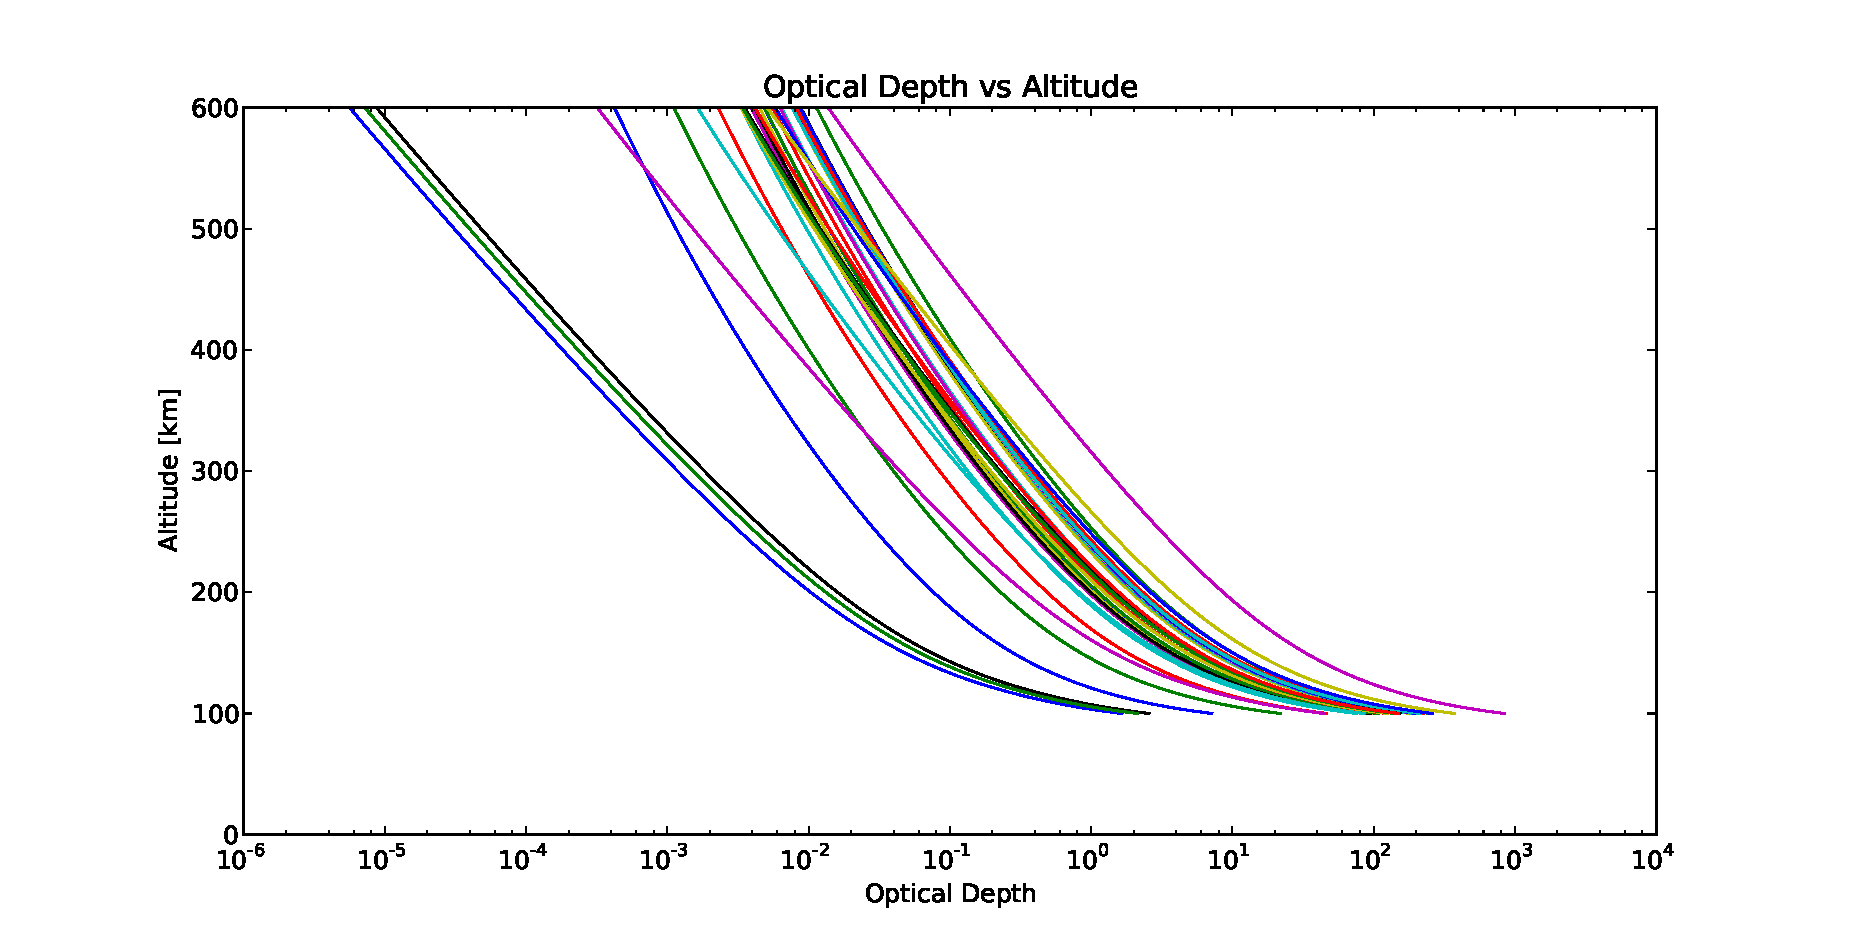
\includegraphics[width=0.5\textwidth]{./Figures/Optical_Depth_vs_Altitude.eps}
	\caption{Optical depths for all 37 wavelengths of the EUVAC solar flux model.}
	\label{fig:optical_depths}
\end{figure}
Next I calculated the intensities of each wavelength and plotted them to get an idea of how they attenuate with depth (Figure~\ref{fig:intensities}).
\begin{figure}[H]
	\centering
		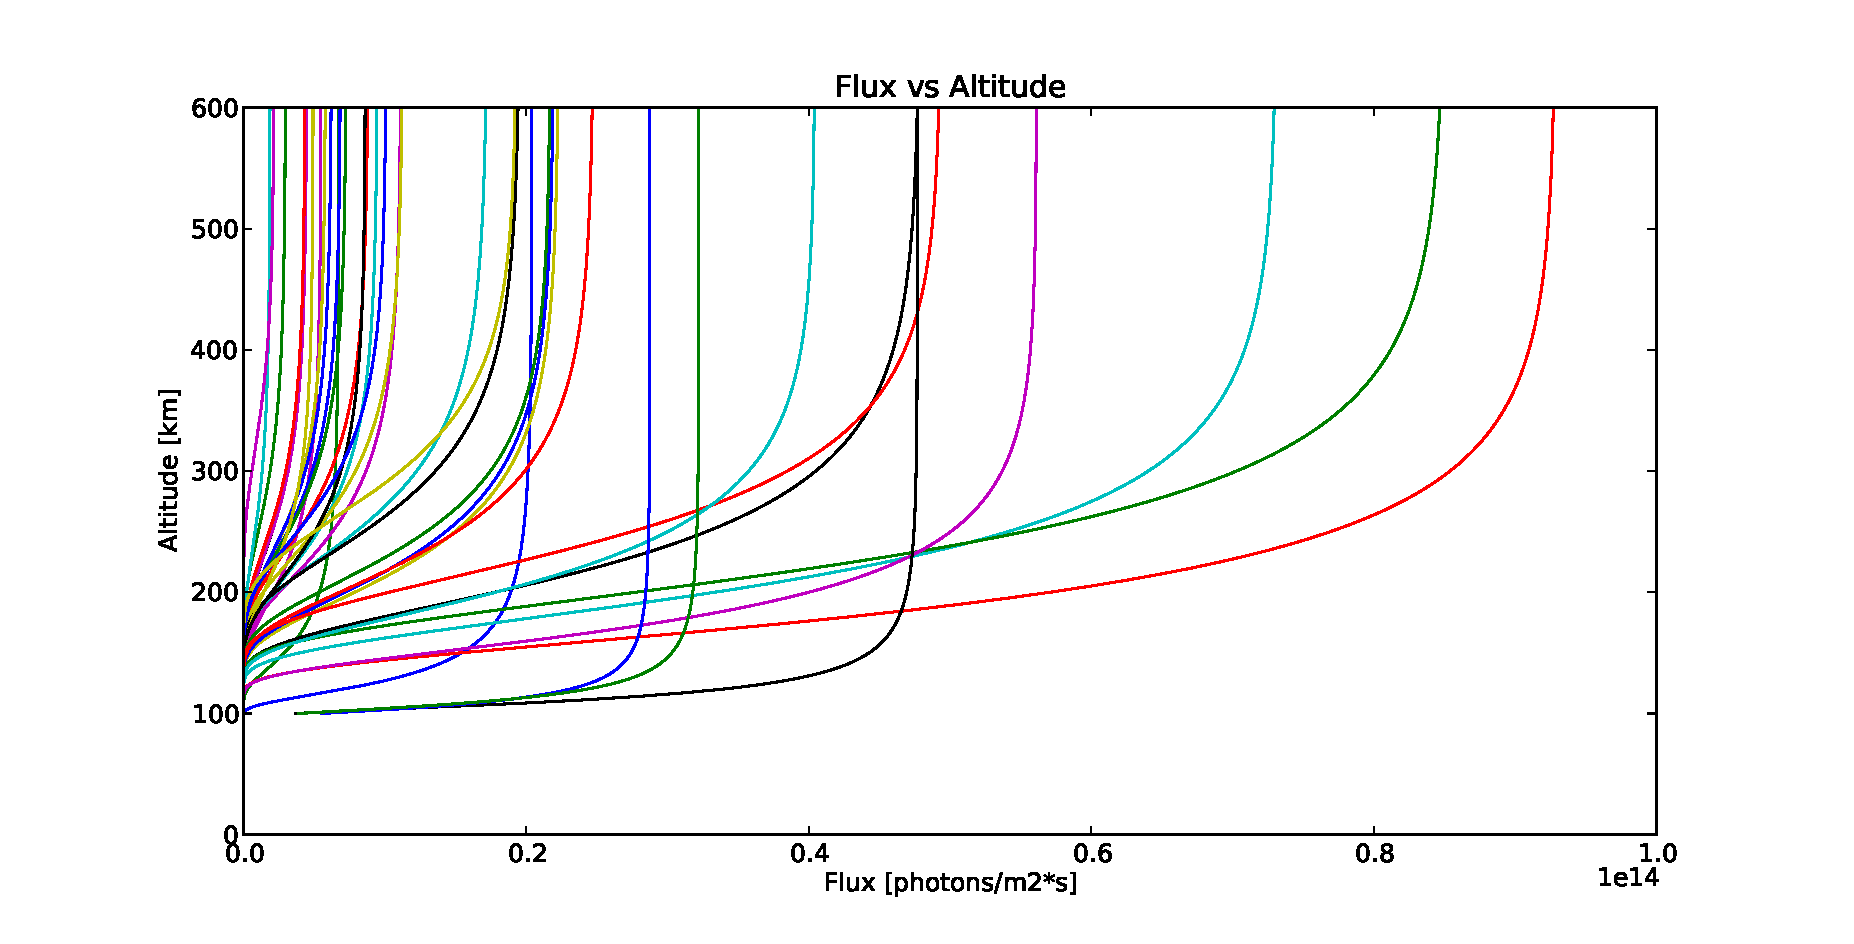
\includegraphics[width=0.5\textwidth]{./Figures/Flux_vs_Altitude.eps}
	\caption{Intensity of each wavelength attenuates with depth.}
	\label{fig:intensities}
\end{figure}
After the calculations for optical deptha and intensity it was fairly simple to calculate the energy dissipation. Plotting the energy dissipation vs altitude (Figure~\ref{fig:energy_dissipation} we find very cool behavior showing that the energy has a peak deposition at two different depths. Since energy deposition is a function of wavelength and number density I believe that it makes sense that the first peak corresponds to where $\tau=1$ for the wavelengths that interact more heavily with one species and the second peak would correspond to $\tau=1$ for the wavelengths that interact more heavily with another. However I am not entirely certain of the optical depth-species relationship or which species these peaks correspond to. One connection I would like to point out is that upon inspecting Figure~\ref{fig:optical_depths} there seems to be two specific peak number of mean free paths traveled for the optical depths. The larger on the order of $10^2$ and the smaller on the order of $10^0$. I believe this also relates to the larger and smaller peaks in the energy dissipation respectively.
\begin{figure}[H]
	\centering
		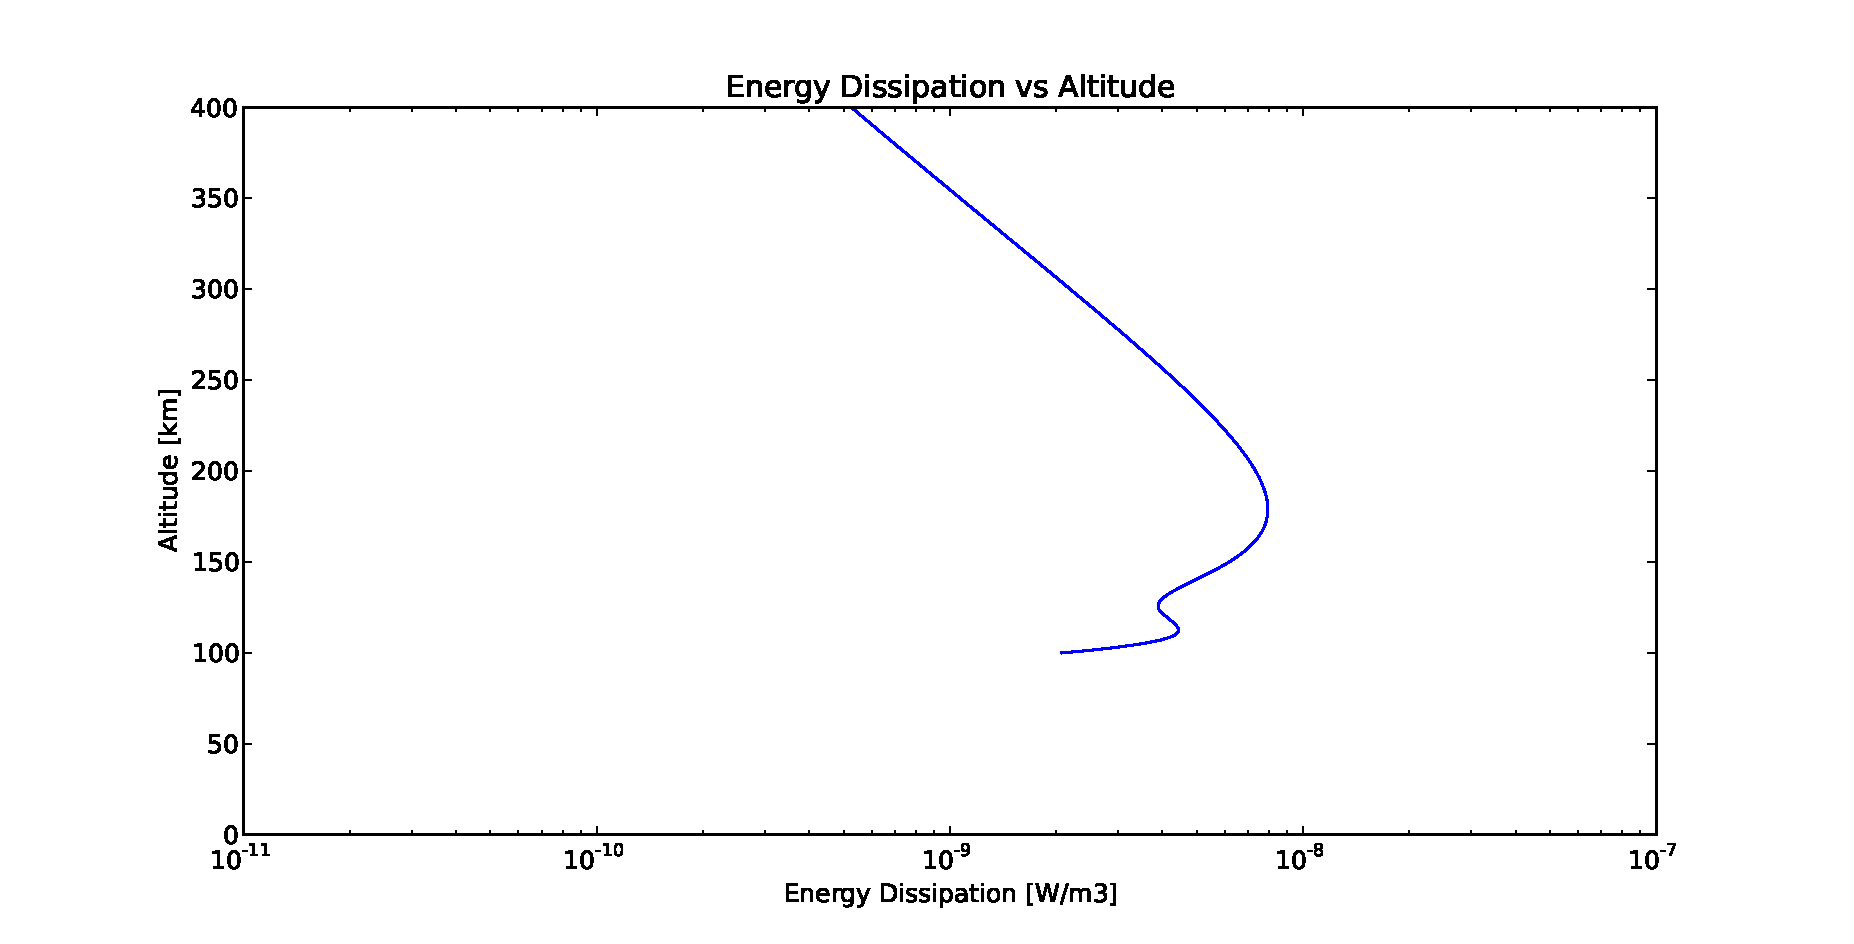
\includegraphics[width=0.5\textwidth]{./Figures/Energy_Dissipation_vs_Altitude.eps}
	\caption{Energy dissipation has two altitude peaks.}
	\label{fig:energy_dissipation}
\end{figure}
While calculating temperature, for every iteration, I asked the computer to plot the new calculated temperature. Figure~\ref{fig:temps} is the result. We can see that initially the temperature jumped around a bit but eventually it began to converge somewhere between 1700K and 1900K.
\begin{figure}[H]
	\centering
		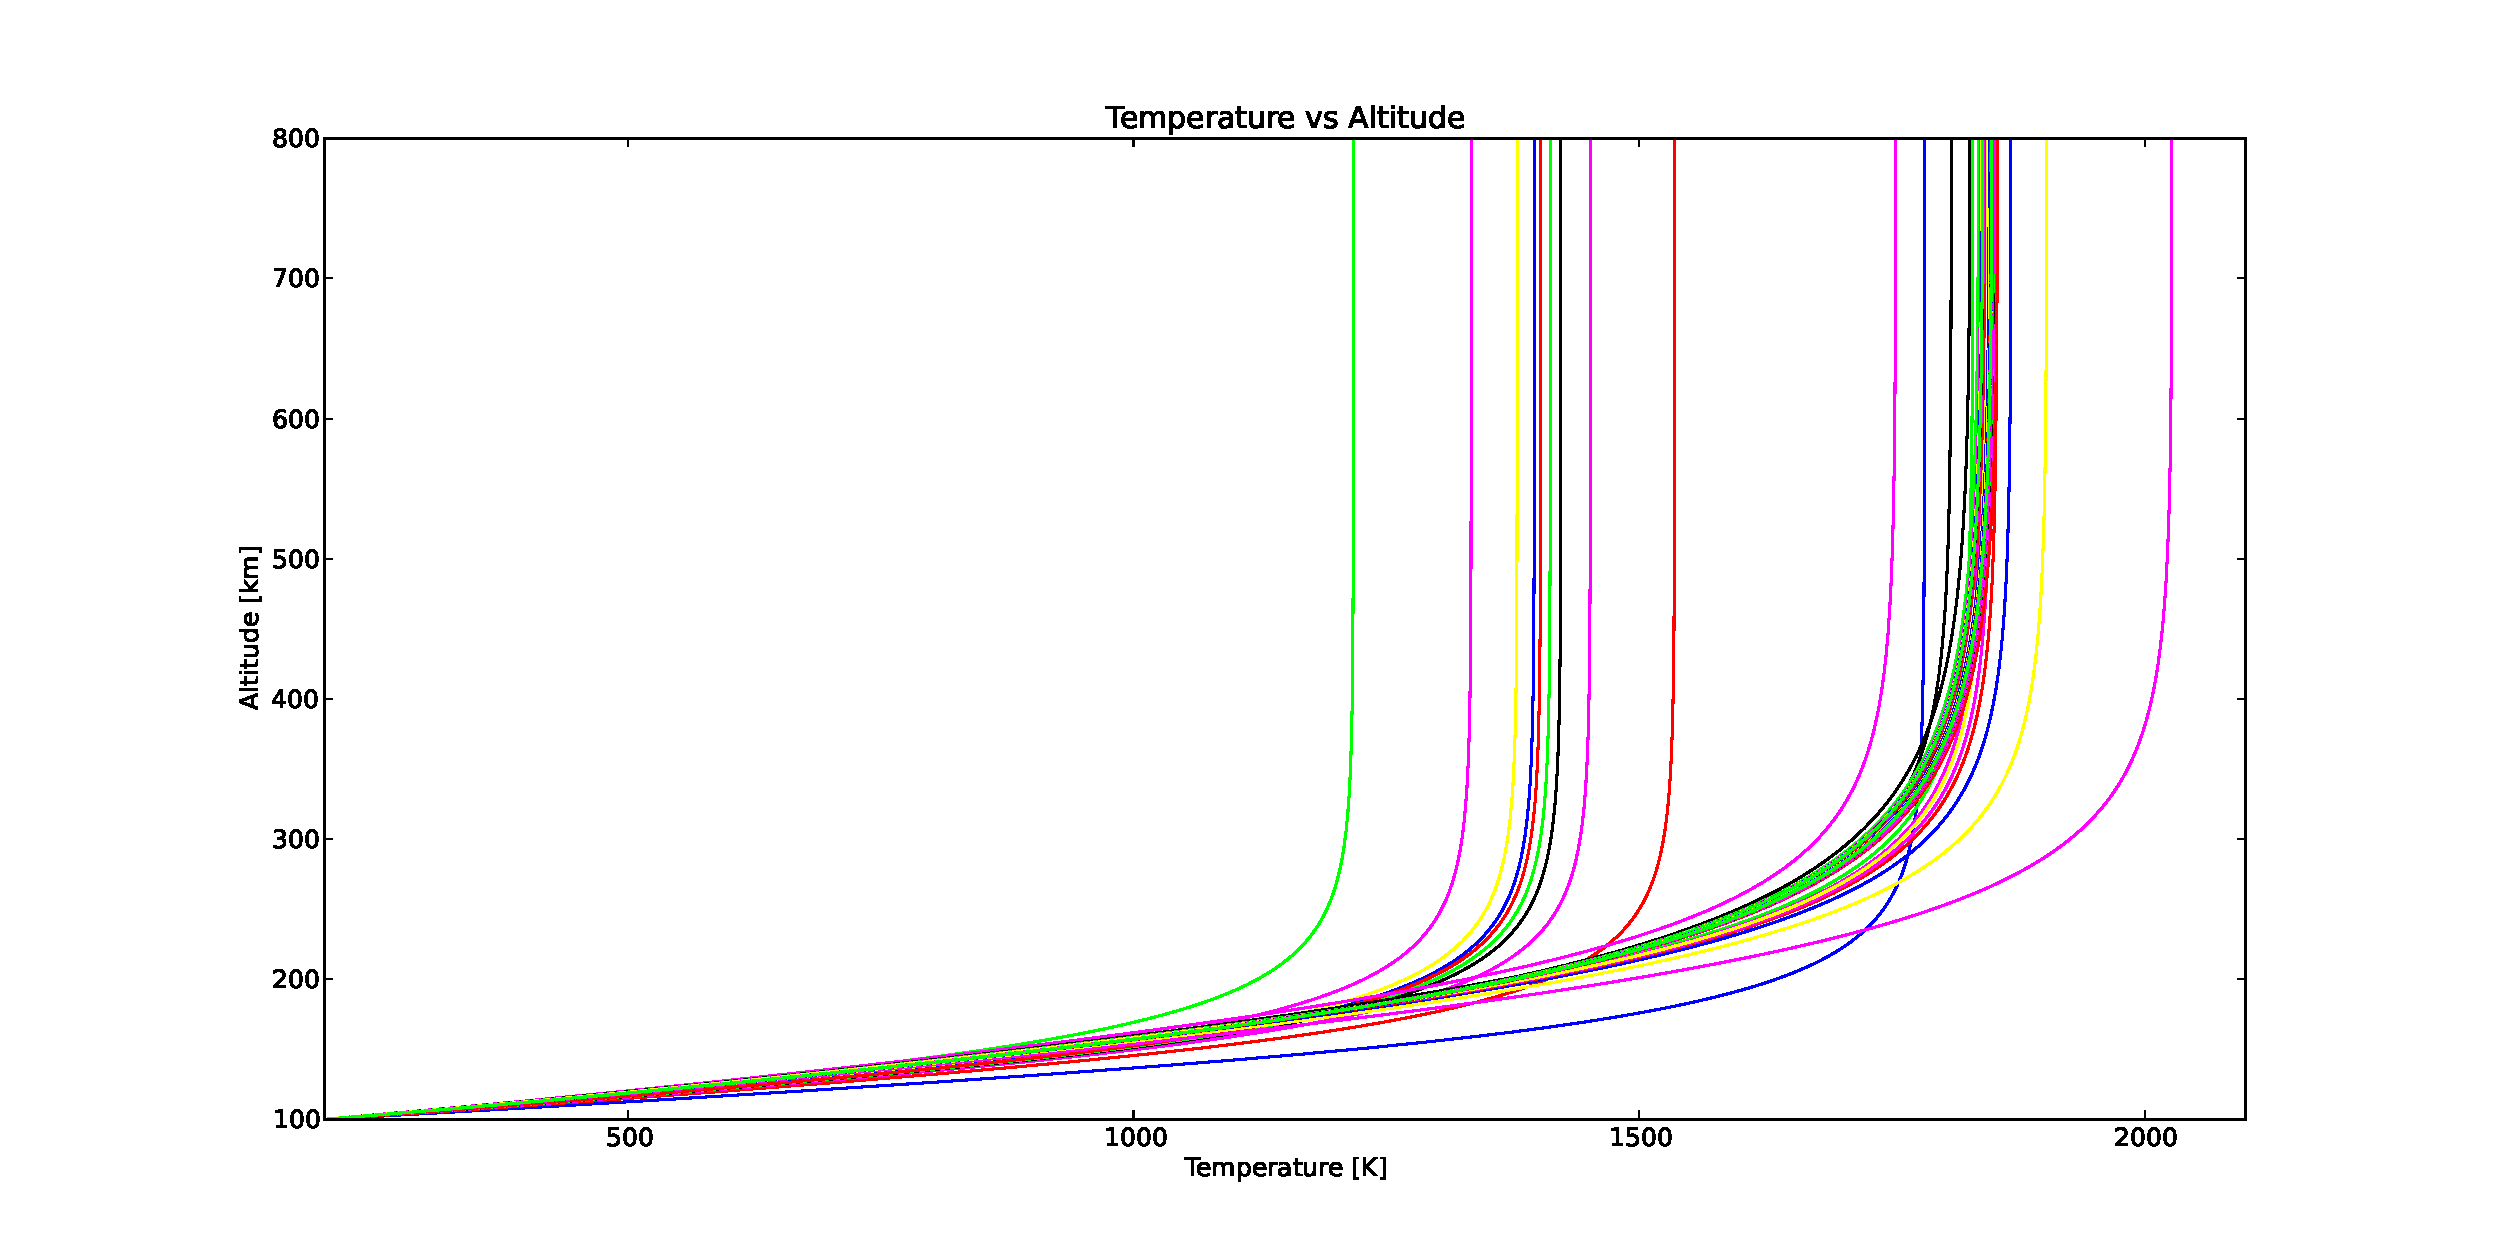
\includegraphics[width=0.5\textwidth]{./Figures/temps.eps}
	\caption{100 iterations of temperature calculations.}
	\label{fig:temps}
\end{figure}
Plotting only the final value of temperature in Figure~\ref{fig:temp} we can see that the thermospheric temperature does in fact converge at 1848K. This is a rather dramatic temperature increase from the initial guess that I used for assignment 1 which was closer to 1100K.
\begin{figure}[H]
	\centering
		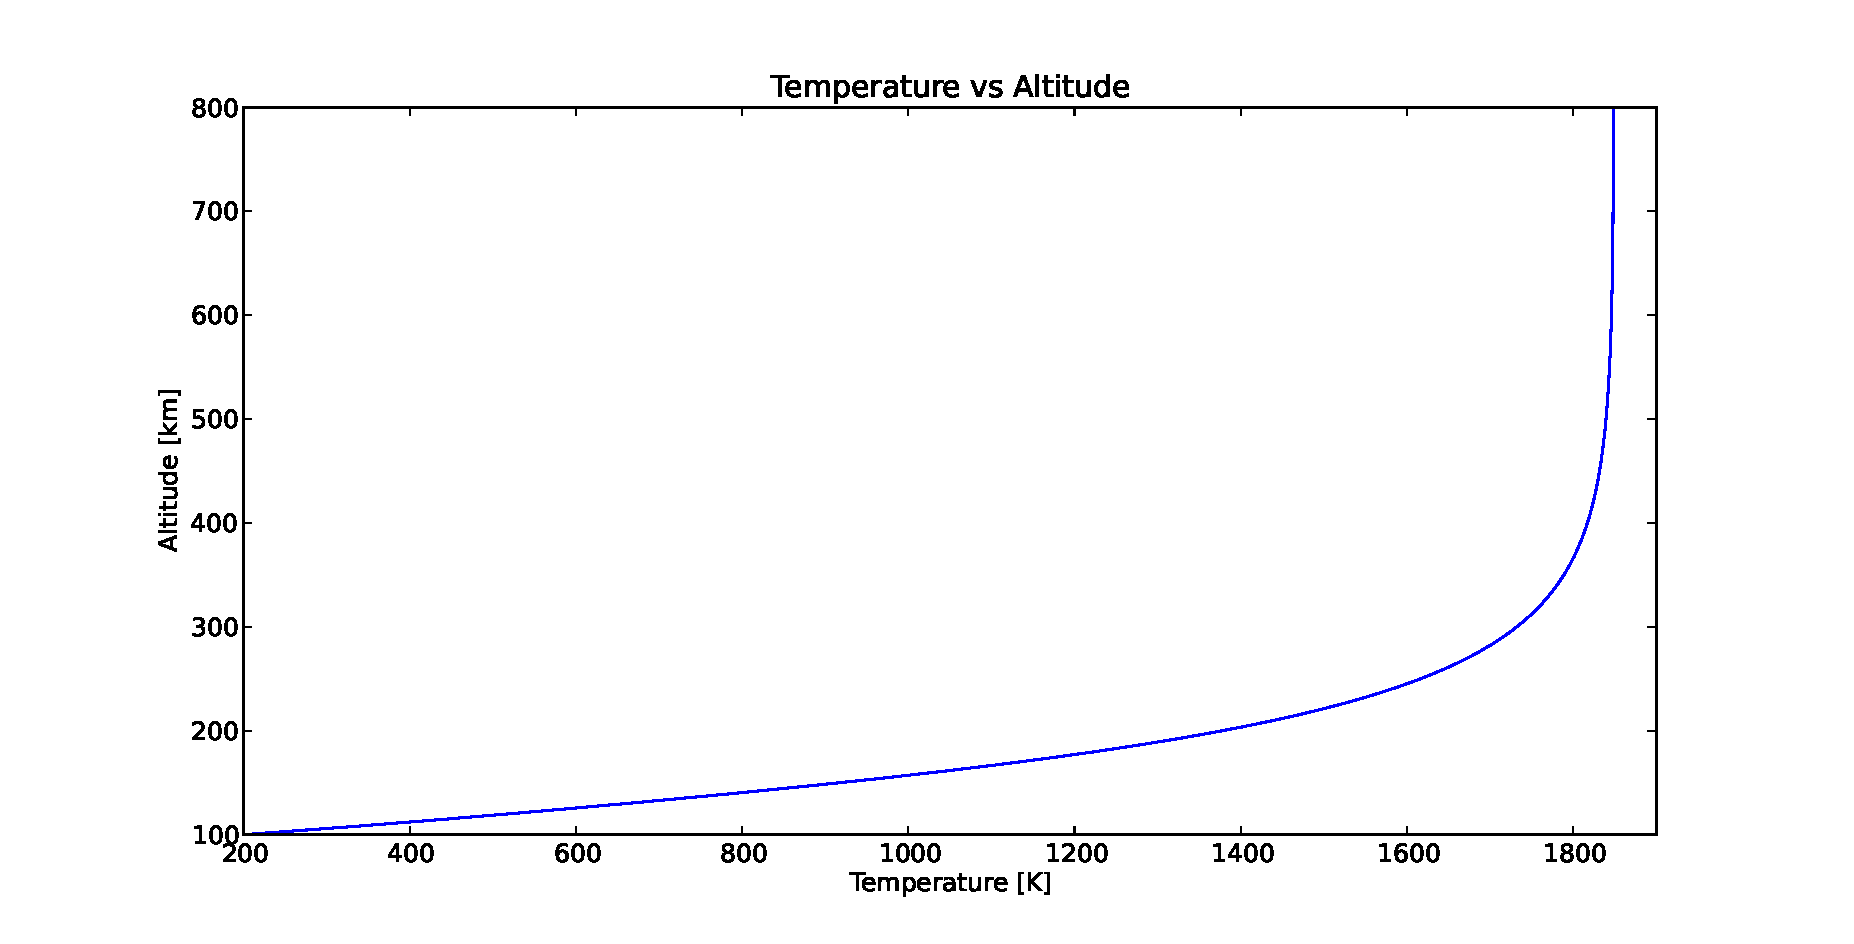
\includegraphics[width=0.5\textwidth]{./Figures/Temperature_vs_Altitude.eps}
	\caption{After 100 iterations of temperature calculations the new temperature profile converges just above 1800K.}
	\label{fig:temp}
\end{figure}
Taking a look at how this new temperature affects the final number density (Figure~\ref{fig:number_density}) we can see that the new number density calculations have steeper curves. This makes sense physically because one would expect that a hotter temperature would give the particles more thermal energy and theus cause the thermosphere to 'puff up'.
\begin{figure}[H]
	\centering
		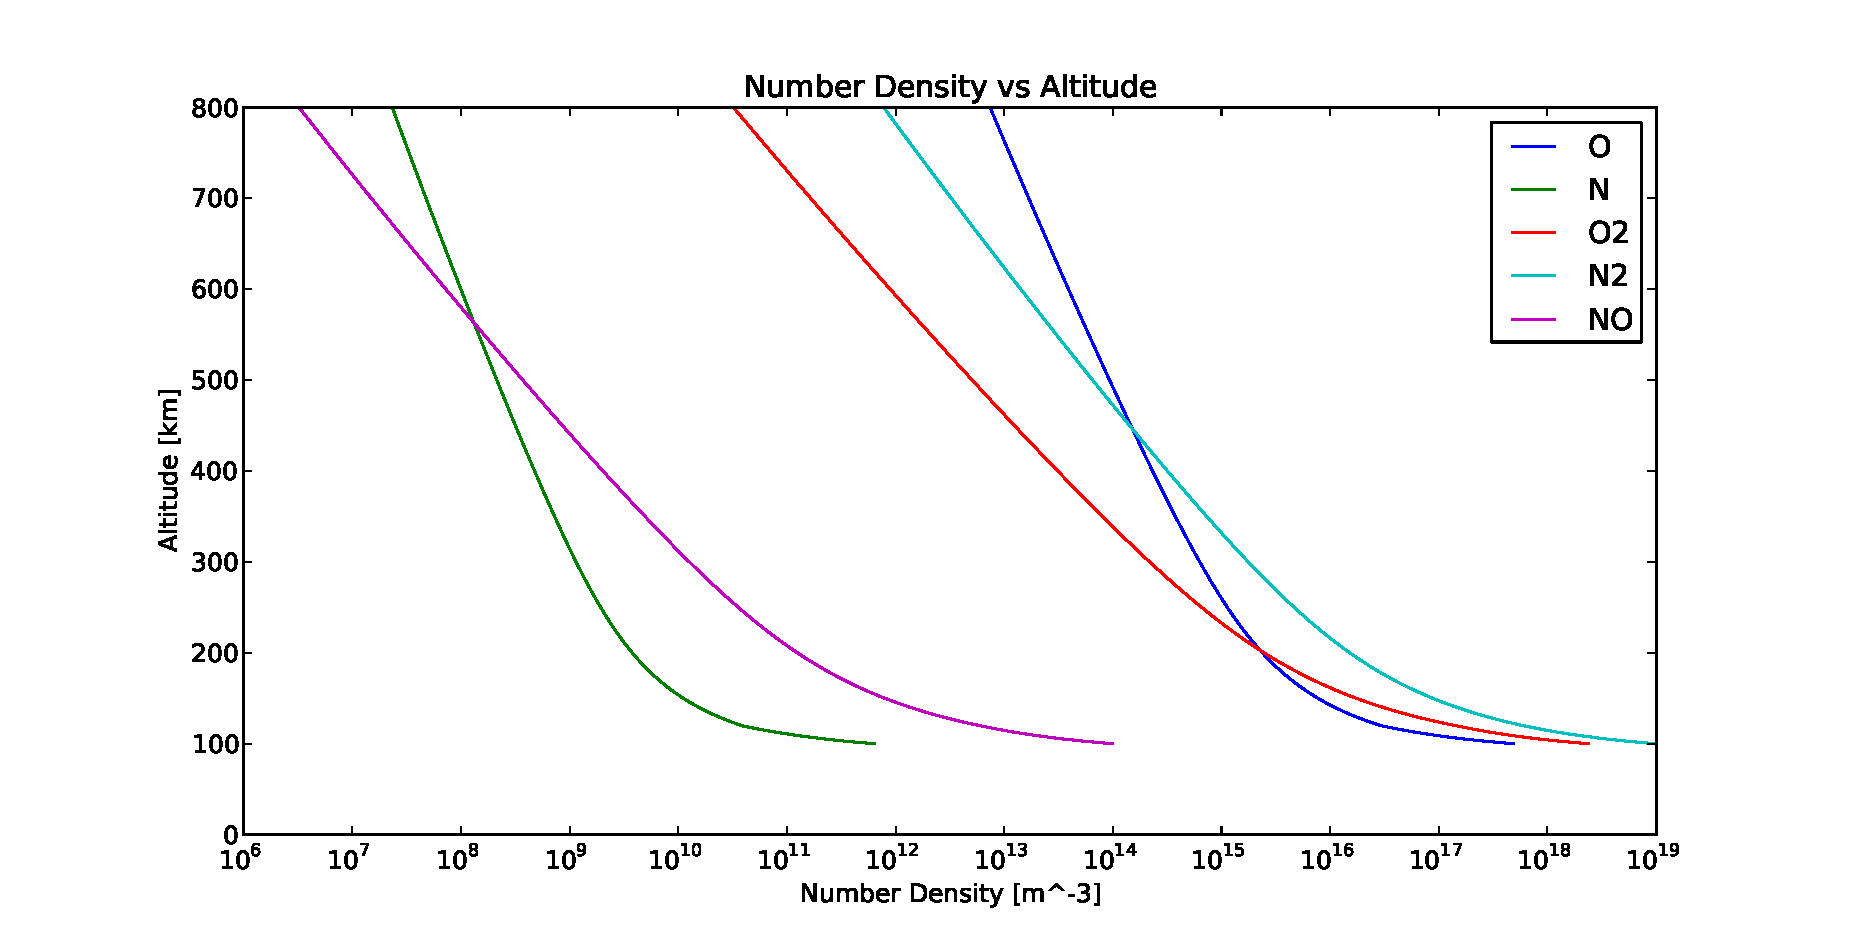
\includegraphics[width=0.5\textwidth]{./Figures/Number_Density_vs_Altitude_100_800.eps}
	\caption{Number density slopes are steeper. The hotter atmosphere is more 'puffy' than before.}
	\label{fig:number_density}
\end{figure}
Previously atmic oxygen became dominant in the atmosphere near 300km (Figure~\ref{fig:O_N_before}) however by Figure~\ref{fig:O_N} we can see that oxygen doesn't become dominant until \raise.17ex\hbox{$\scriptstyle\sim$}450km (Figure~\ref{fig:O_N}).
\begin{figure}[H]
	\centering
		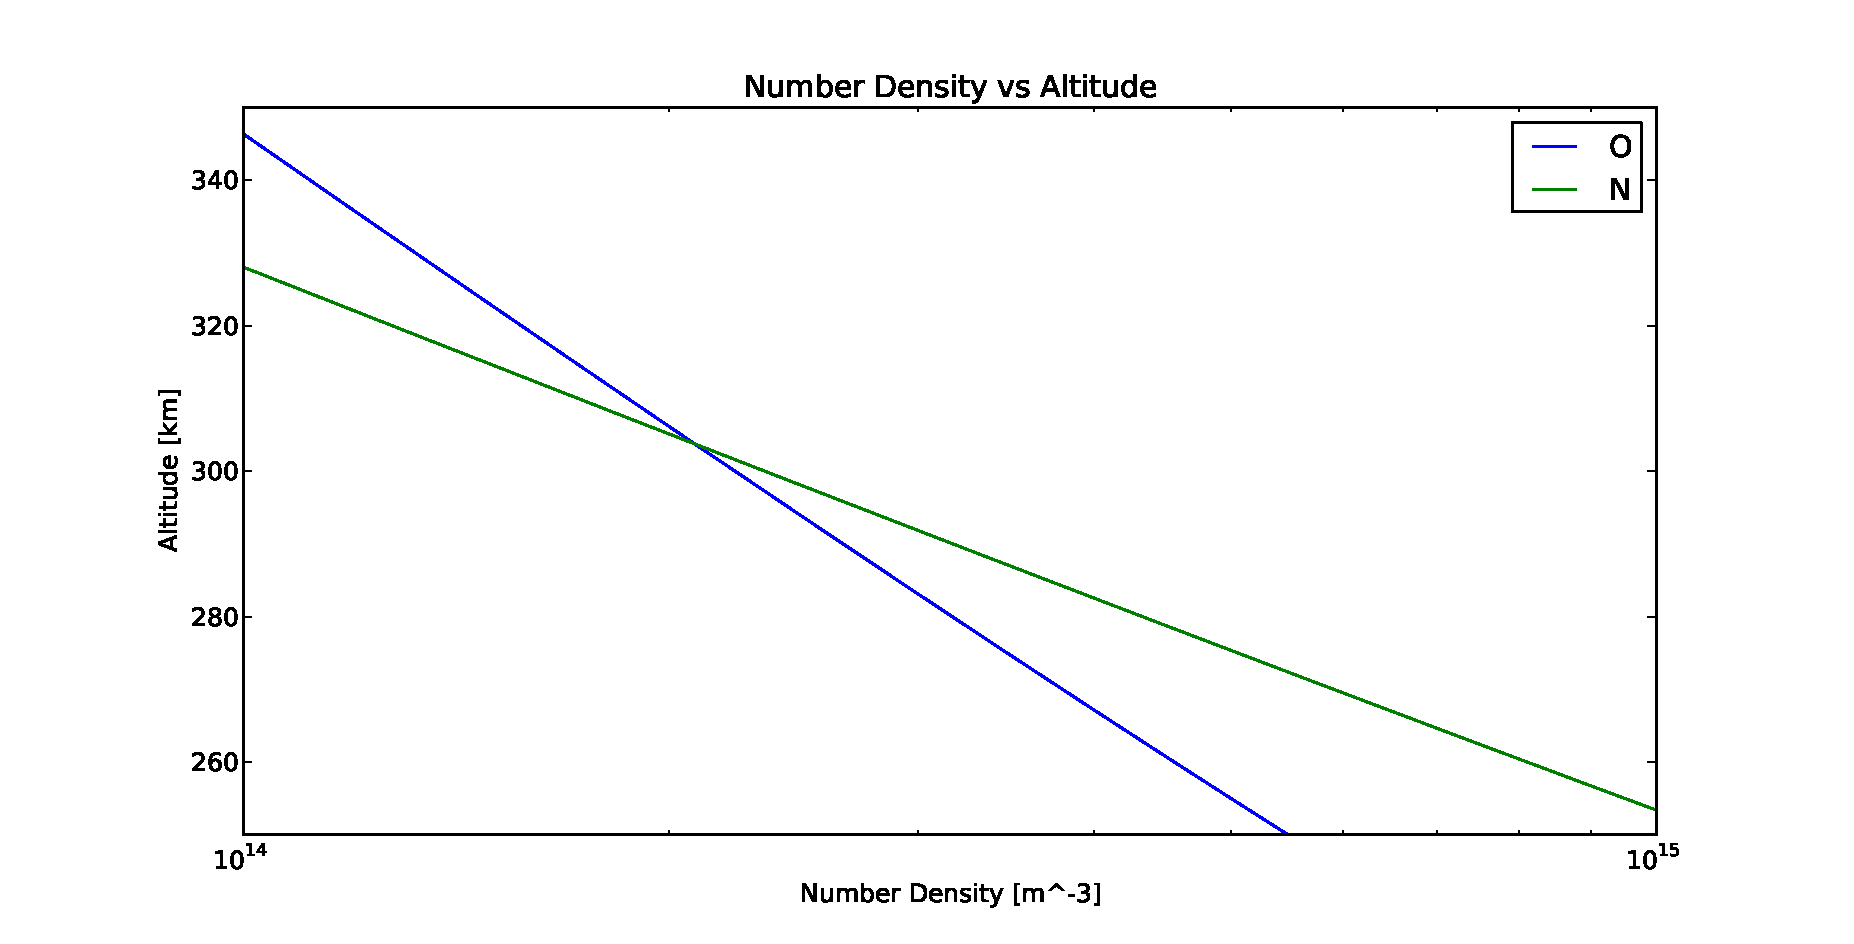
\includegraphics[width=0.5\textwidth]{./Figures/Number_Density_vs_Altitude_Before.eps}
	\caption{With my initial guess at temperature from assignment 1 oxygen became dominant at \raise.17ex\hbox{$\scriptstyle\sim$}300km.}
	\label{fig:O_N_before}
\end{figure}
\begin{figure}[H]
	\centering
		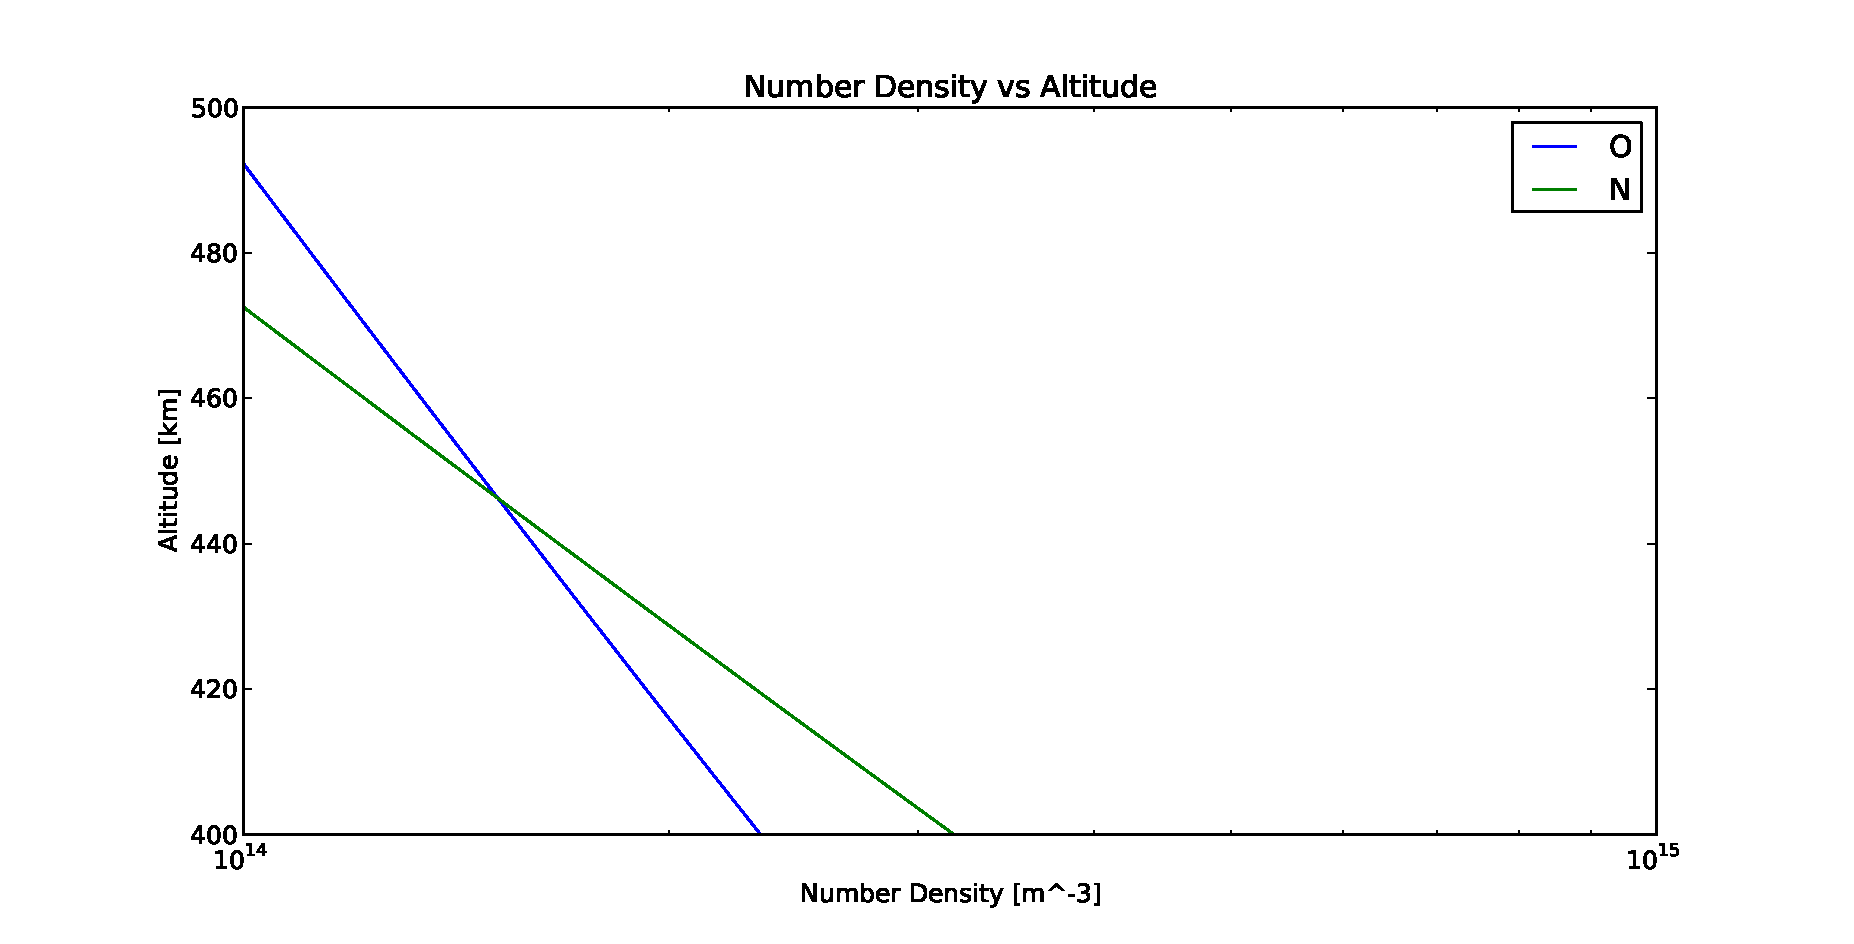
\includegraphics[width=0.5\textwidth]{./Figures/Number_Density_vs_Altitude_400_500.eps}
	\caption{With my new temperature calculation oxygen doesn't become dominant until higher latitude.}
	\label{fig:O_N}
\end{figure}
In Figure~\ref{fig:scale_height} we see that the scale heights maintain the same shape as before but now they are considerably larger. 
\begin{figure}[H]
	\centering
		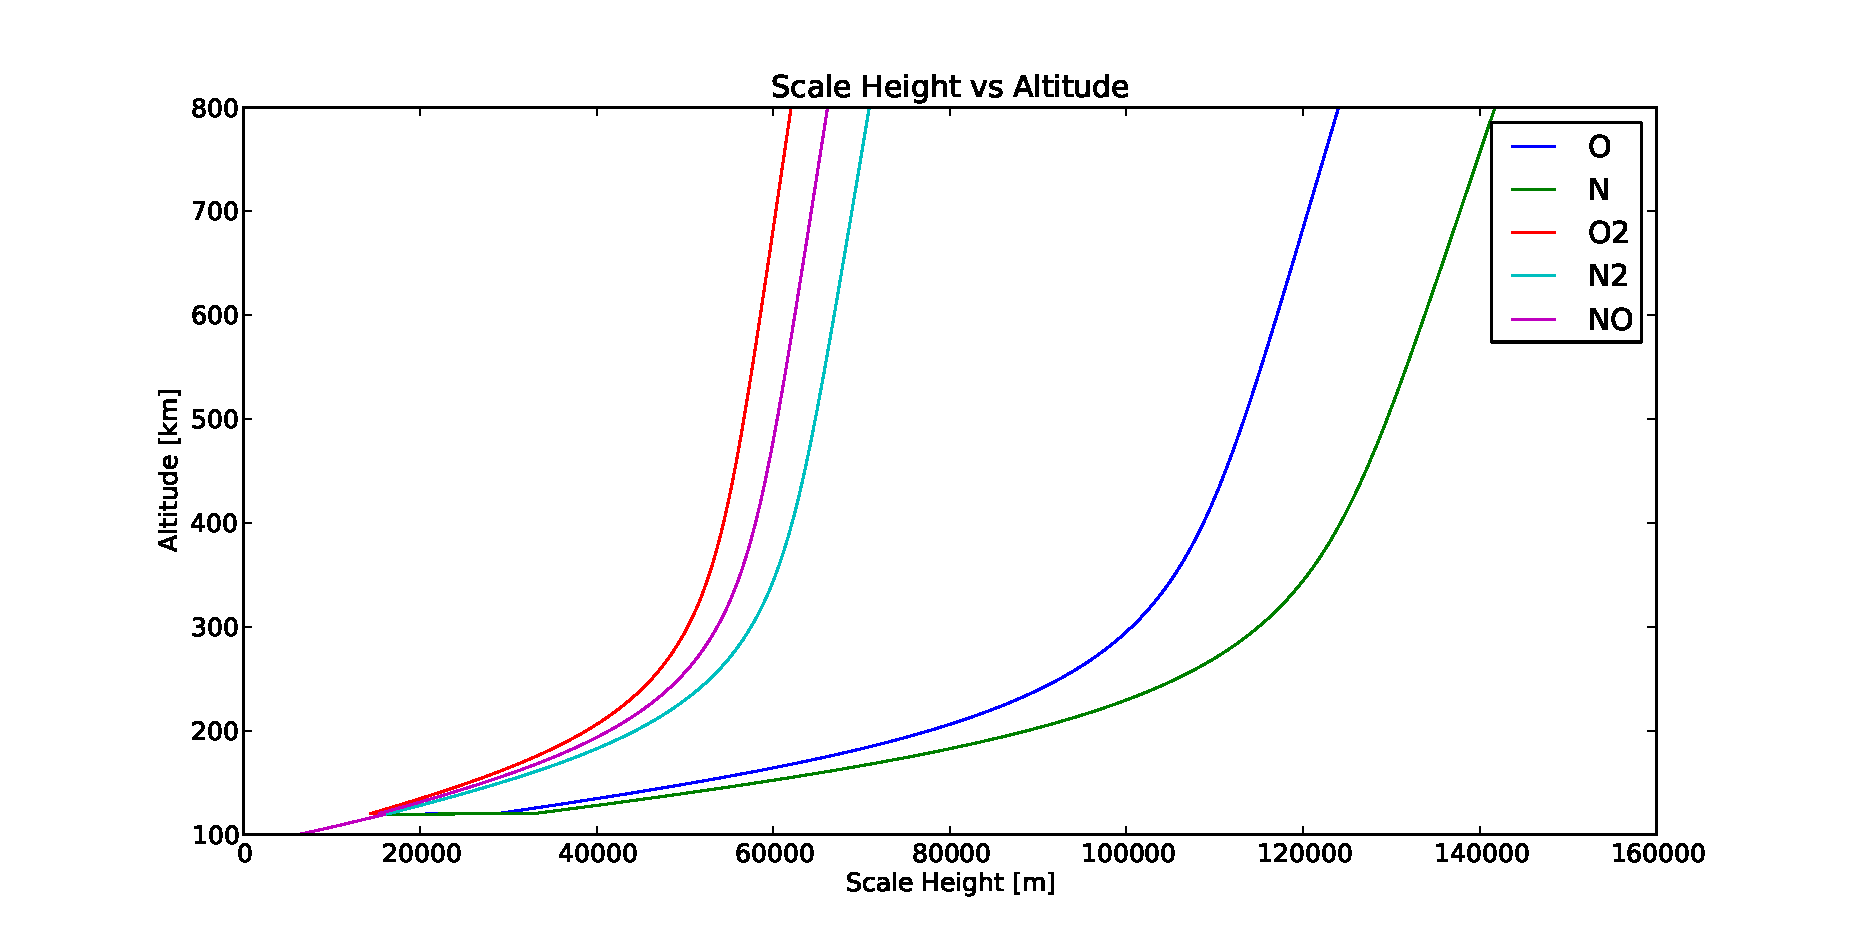
\includegraphics[width=0.5\textwidth]{./Figures/Scale_Height_vs_Altitude.eps}
	\caption{Larger scale heights.}
	\label{fig:scale_height}
\end{figure}
Previously in homework 1 the total weighted molecular mass approached 16amu in the altitude interval in question. Since the atmosphere is hotter and the scale heights are much larger now you can see that in the weighted molecular mass only gets down to about 18amu in the altitude interval (Figure~\ref{fig:molecular_mass}).
\begin{figure}[H]
	\centering
		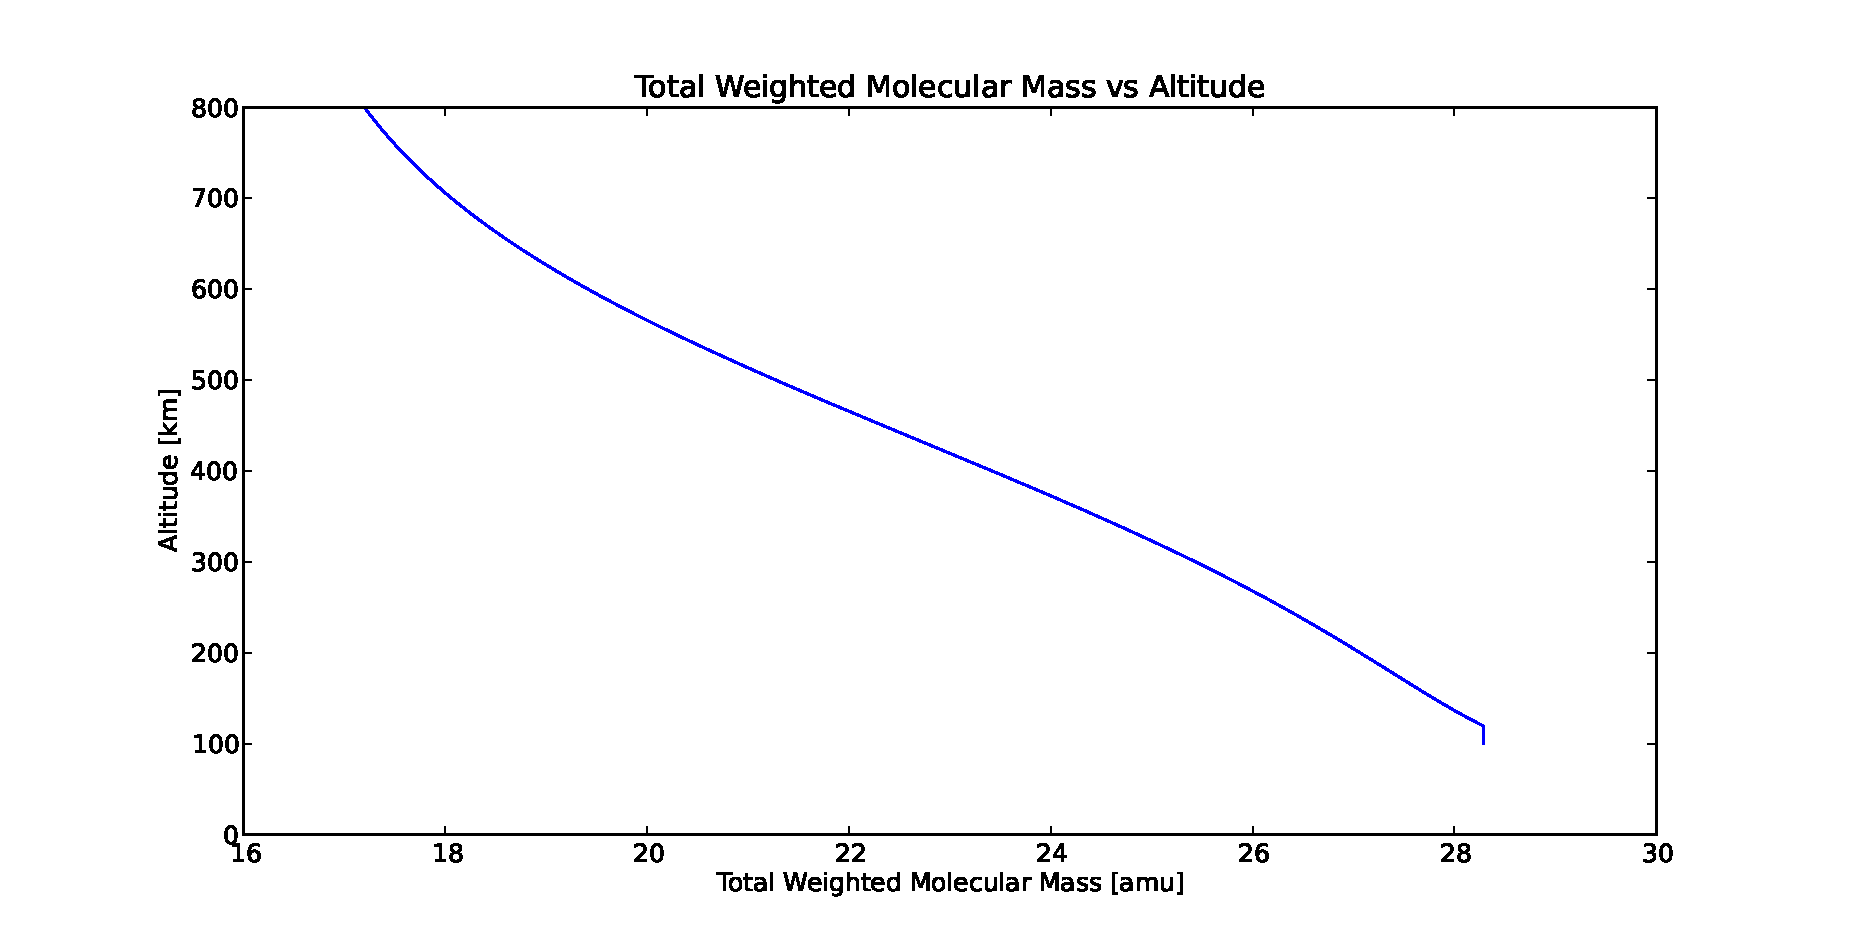
\includegraphics[width=0.5\textwidth]{./Figures/Total_Weighted_Molecular_Mass_vs_Altitude.eps}
	\caption{Total weighted molecular mass only gets down to about 18amu in the altitude range.}
	\label{fig:molecular_mass}
\end{figure}
Similrly to the number density, the mass density followed the same trend (Figure~\ref{fig:mass_density}).
\begin{figure}[H]
	\centering
		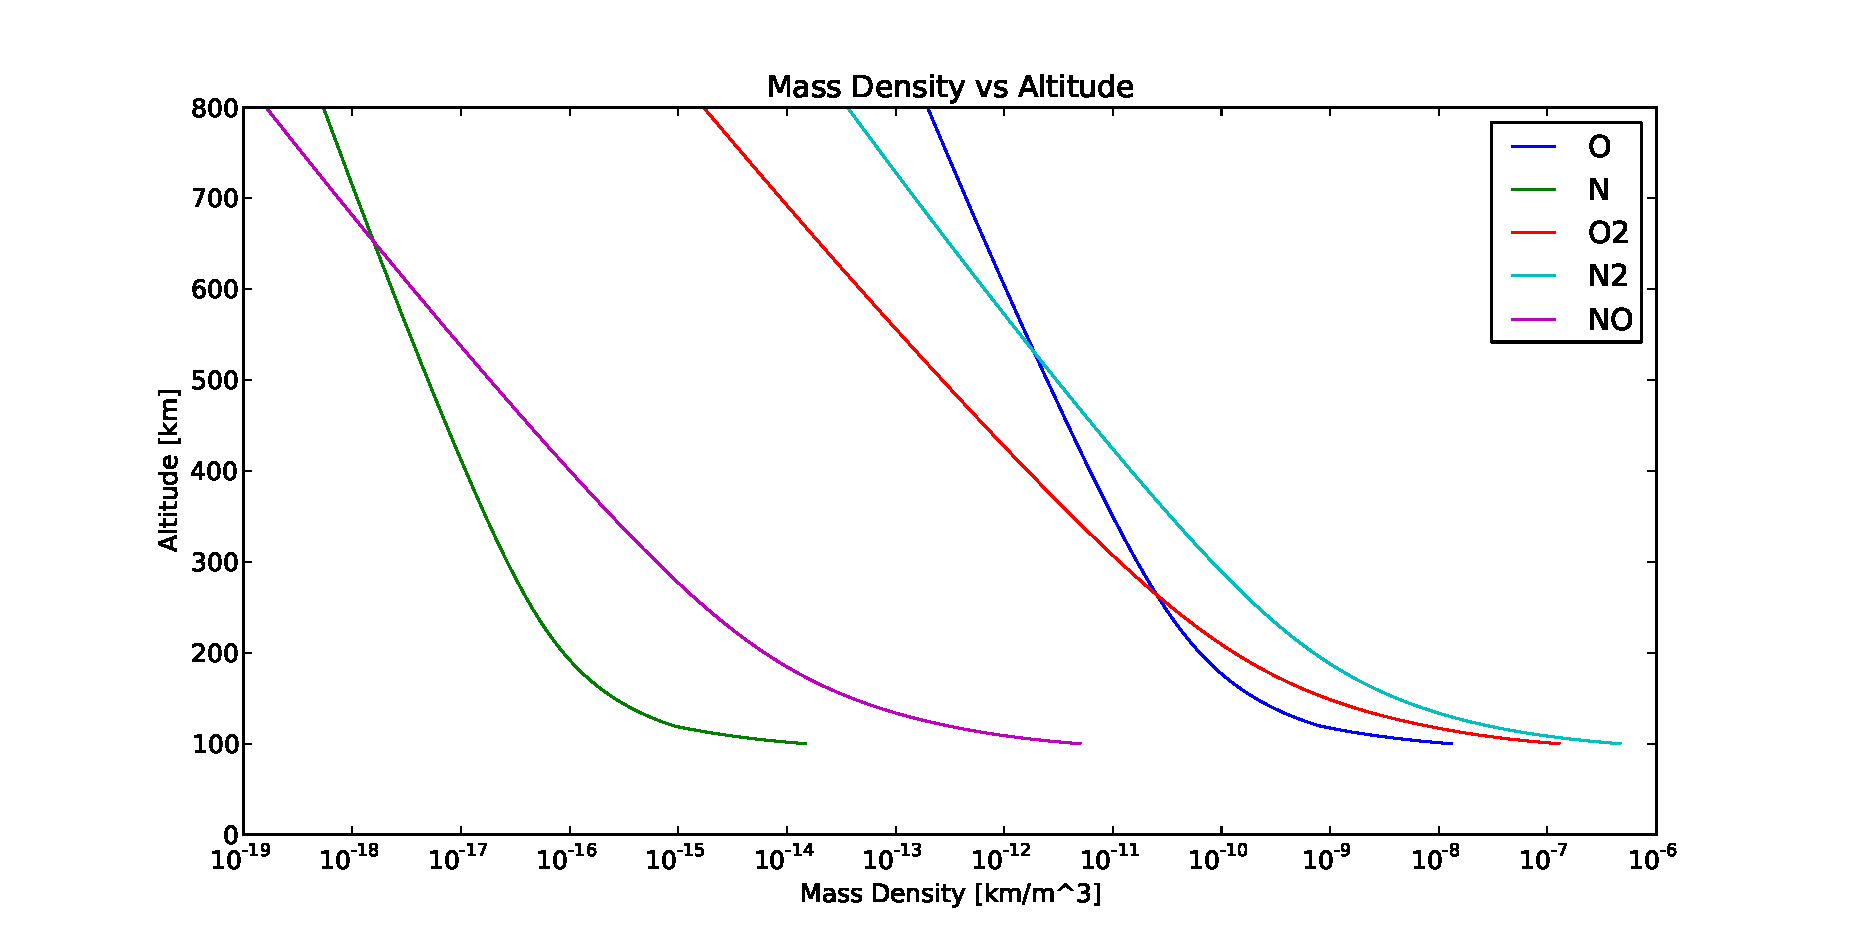
\includegraphics[width=0.5\textwidth]{./Figures/Mass_Density_vs_Altitude.eps}
	\caption{Mass density also has a steeper slope.}
	\label{fig:mass_density}
\end{figure}
In calculating the optical depth we essentially had to calculate the column number density. Figure~\ref{fig:column_number} is a plot of column density vs altitude. Not too surprisingly it behaves similarly to number density and mass density.
\begin{figure}[H]
	\centering
		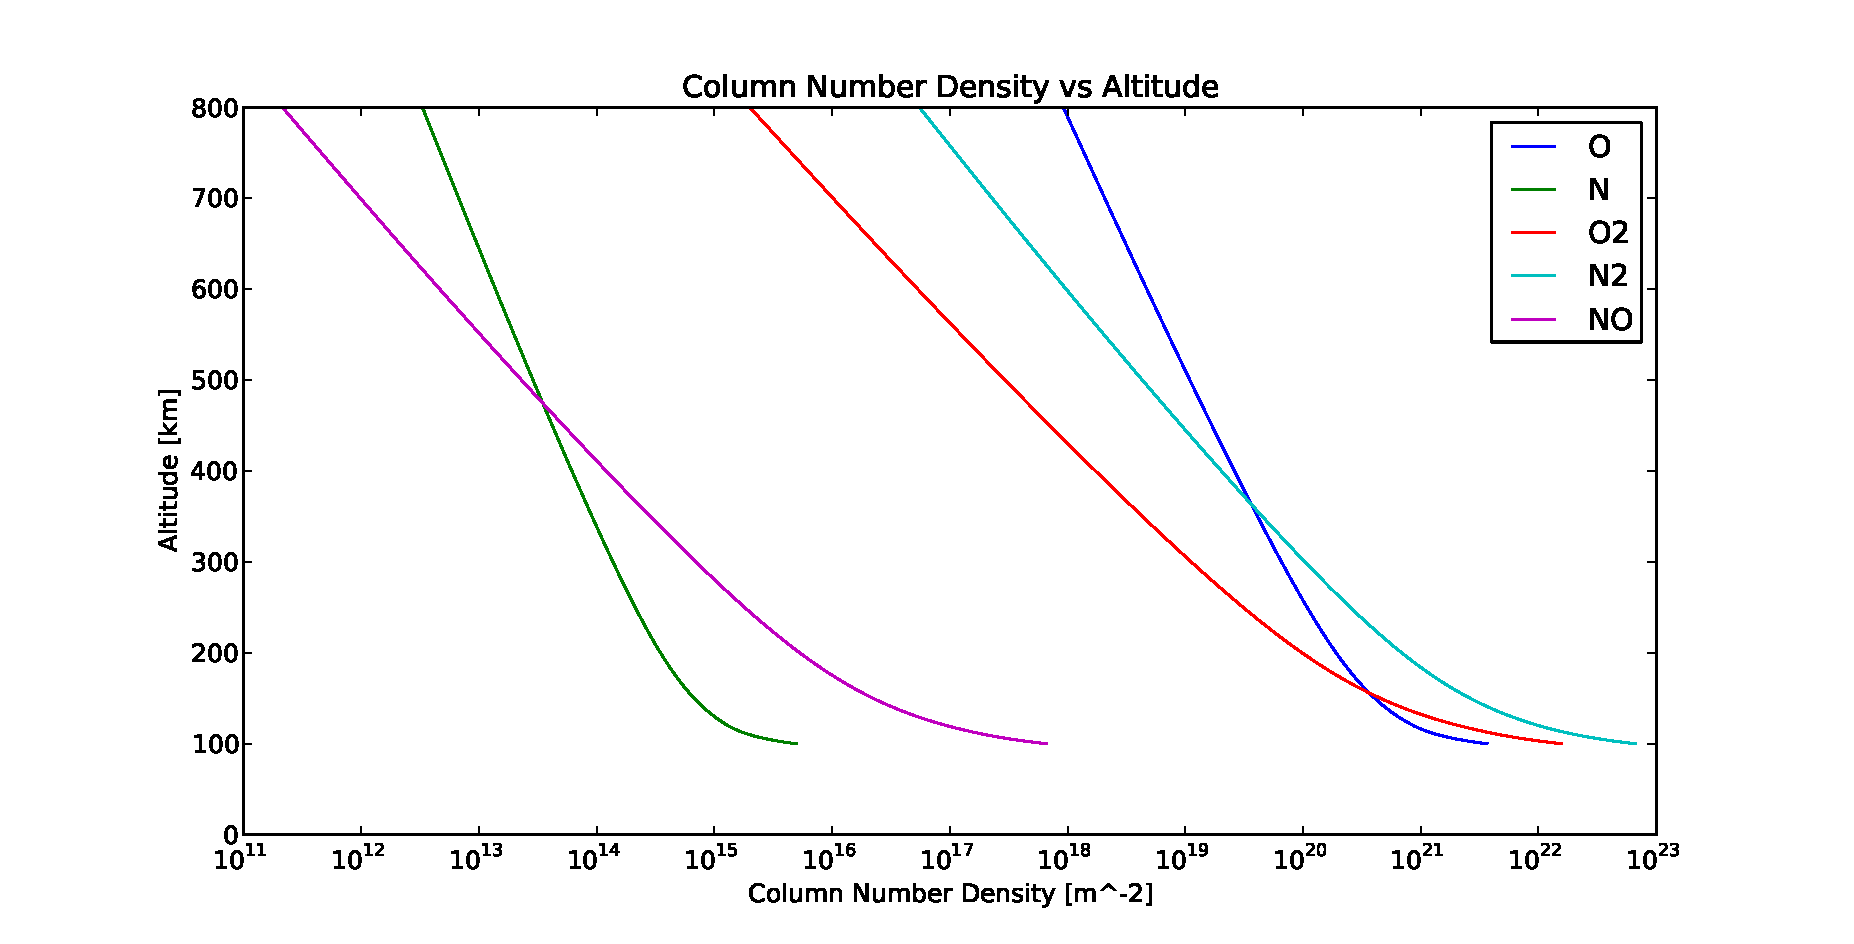
\includegraphics[width=0.5\textwidth]{./Figures/Column_Number_Density_vs_Altitude.eps}
	\caption{Column number density behaves simlarly to number density (same general trend in the curves).}
	\label{fig:column_number}
\end{figure}
Likewise I thought it would be important to also show the column mass density vs altitude (Figure~\ref{fig:column_mass}).
\begin{figure}[H]
	\centering
		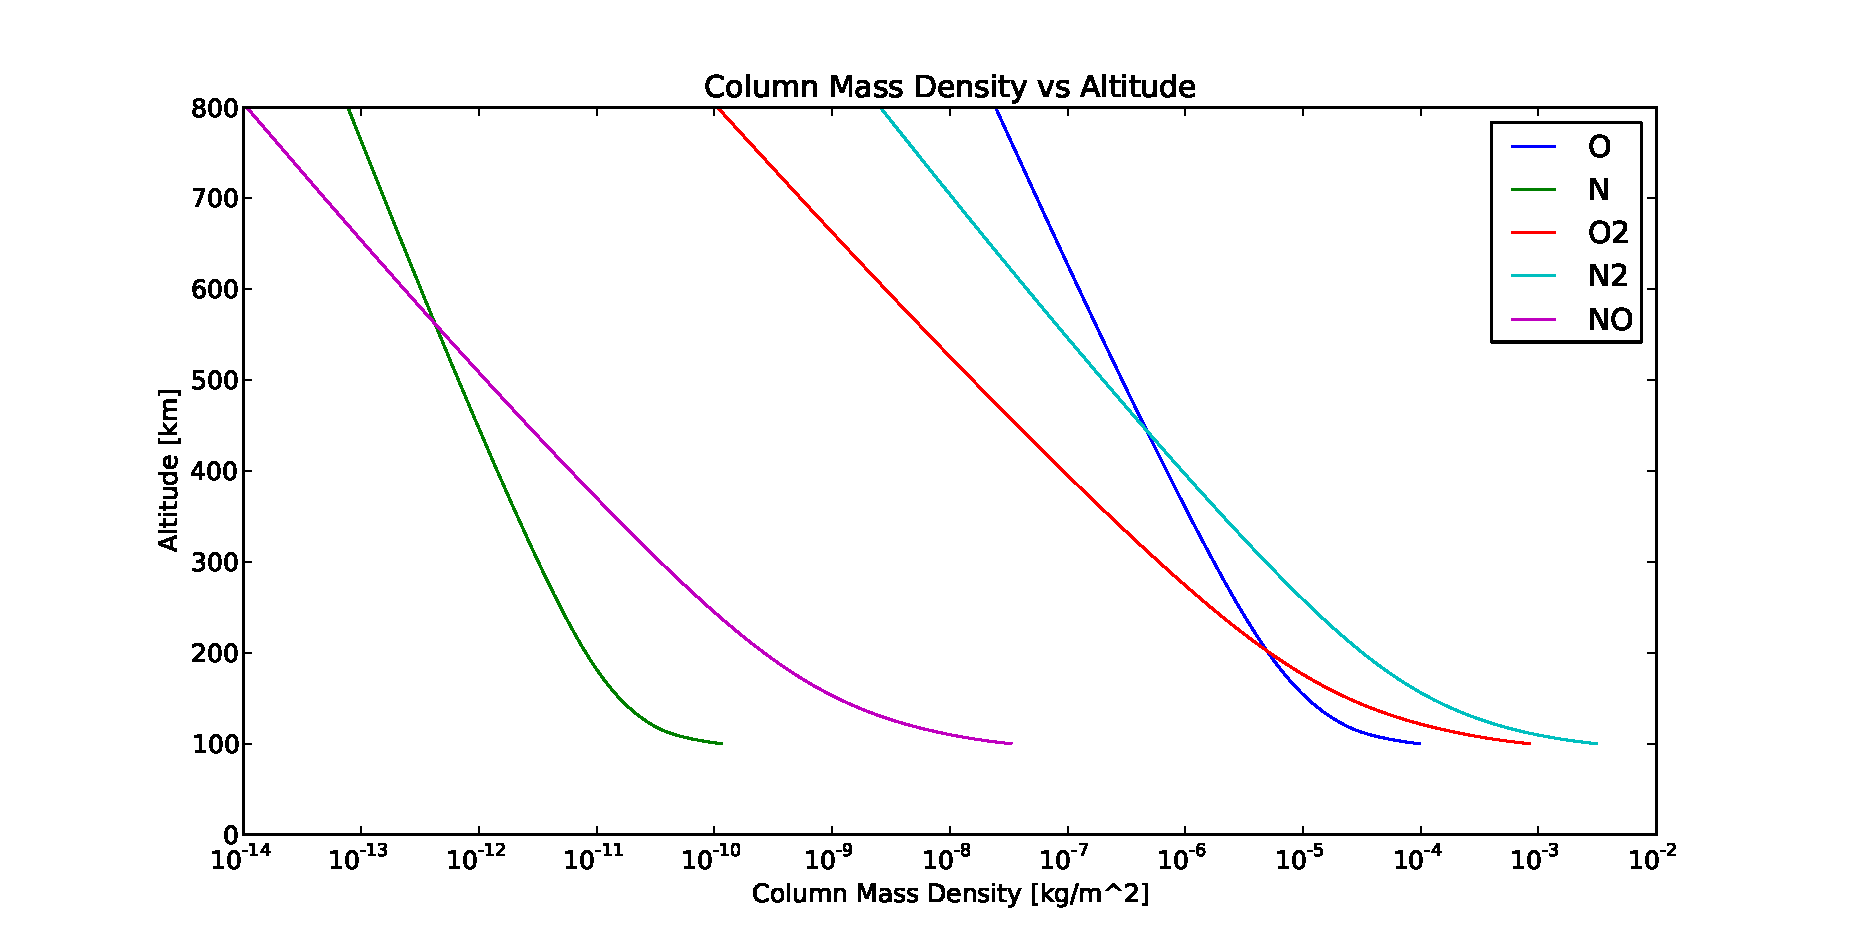
\includegraphics[width=0.5\textwidth]{./Figures/Column_Mass_Density_vs_Altitude.eps}
	\caption{Column mass density behaves similarly to mass density (same general trend in the curves).}
	\label{fig:column_mass}
\end{figure}



\section{Conclusion}
It is clear by this exercise that the behavior of the thermosphere is highly dependent upon temperature. Temperature is driven by solar intensity. So the more incoming radiation the atmosphere recieves the hotter the thermosphere will get driving the molecular diffusion process to higher altitudes. It is important to not that while the new added physics made the thermosphere more 'realistic' in some sense it is important to note that we are only considering the source term. To get a more accurate temperature profile we should consider loss/cooling processes via chemistry.



\end{multicols}
\end{document}
